\documentclass[../main]{subfiles}
\begin{document}
\chapter{Trees and Ensemble Learning}
\begin{introduction}
    \item Decision Trees and Axis-Aligned Splits
    \item Information Gain and Mutual-Information
    \item Feature Selection and Purity Measures
    \item Bagging and Variance Reduction
    \item Random Forests and Out-of-Bag Evaluation
    \item Boosting and Functional Gradient View
\end{introduction}

\section{Review: Gaussian Processes and Bayesian Optimization}

In the previous chapter, we introduced Gaussian Processes (GPs) and showed how
they can be used for regression.  Given training inputs
\begin{equation}
    X = (x_1,\dots,x_n), \qquad
    y = (y_1,\dots,y_n)^\top,
\end{equation}
and a test point $x_\star$, a GP prior with kernel $k(\cdot,\cdot)$ and i.i.d.\
Gaussian observation noise of variance $\lambda$ yields the joint Gaussian
distribution
\begin{equation}
    \begin{pmatrix}
        y\\[2pt]
        f_\star
    \end{pmatrix}
    \sim
    \mathcal{N}\!\left(
        0,\,
        \begin{bmatrix}
            K(X,X) + \lambda I_n
            & k(X,x_\star)\\[2pt]
            k(x_\star,X) & k(x_\star,x_\star)
        \end{bmatrix}
    \right),
\end{equation}
where $K(X,X)$ is the $n\times n$ Gram matrix and
$k(X,x_\star) = (k(x_1,x_\star),\dots,k(x_n,x_\star))^\top$.
Conditioning on the observed $y$ gives the posterior predictive distribution
for $f_\star = f(x_\star)$:
\begin{align}
    \mu_\star
    &= \mathbb{E}[f_\star \mid X,y,x_\star]
      = k(x_\star,X)^\top
        \bigl(K(X,X)+\lambda I_n\bigr)^{-1} y,
        \label{eq:gp-posterior-mean}\\
    \sigma_\star^2
    &= \operatorname{Var}[f_\star \mid X,y,x_\star]
      = k(x_\star,x_\star)
        - k(x_\star,X)^\top
          \bigl(K(X,X)+\lambda I_n\bigr)^{-1}
          k(x_\star,X).
        \label{eq:gp-posterior-var}
\end{align}
By evaluating $\mu_\star$ at many test points and optionally plotting
$\mu_\star \pm \sigma_\star$, we obtain a smooth predictive curve together with
credible intervals that quantify uncertainty.

\subsection{Black-Box Optimization with Gaussian Processes}

An important application of GP regression is \emph{Bayesian Optimization} (BO),
which addresses \emph{black-box optimization} problems:
\begin{equation}
    \max_{x\in\mathcal{X}} f(x),
\end{equation}
where:
\begin{itemize}
    \item $f(x)$ has no known analytic form (no closed-form expression);
    \item gradients $\nabla f(x)$ are unavailable;
    \item each evaluation of $f(x)$ is \emph{expensive}.
\end{itemize}
We can, however, query the black box at chosen points:
\begin{equation}
    y = f(x) + \varepsilon,
\end{equation}
and use these point evaluations to build a surrogate model.

A canonical example is \emph{hyperparameter tuning} for neural networks or
other machine learning models.  Here:
\begin{itemize}
    \item $x$ encodes a vector of hyperparameters (learning rate, width, depth,
    regularization strength, \dots);
    \item $f(x)$ is the validation performance (e.g.\ accuracy) obtained by
    training the model with hyperparameters $x$ and evaluating on a validation
    set.
\end{itemize}
Each function evaluation requires a full train--validate cycle and is therefore
very costly, so we must find good $x$ using as \emph{few} evaluations as
possible.

\begin{remark}[Basic Bayesian Optimization Loop]
    Bayesian Optimization with a GP surrogate proceeds iteratively:
    \begin{enumerate}
        \item \textbf{Initialization.}  Select an initial design
        $\{x_i\}_{i=1}^n$ (e.g.\ random or space-filling) and evaluate
        $y_i = f(x_i)$.
        \item \textbf{Fit GP surrogate.}  Use $\{(x_i,y_i)\}_{i=1}^n$ to fit a GP
        regression model, yielding posterior mean $\mu(x)$ and variance
        $\sigma^2(x)$ for all $x\in\mathcal{X}$.
        \item \textbf{Acquisition maximization.}  Define an \emph{acquisition
        function} $a(x)$ that uses $\mu(x)$ and $\sigma(x)$ to score candidate
        points, and choose the next evaluation point(s) by
        \begin{equation}
            x_{\text{next}} \in \argmax_{x\in\mathcal{X}} a(x).
        \end{equation}
        \item \textbf{Evaluate and update.}  Query the black box at
        $x_{\text{next}}$ to obtain $y_{\text{next}} = f(x_{\text{next}})$, augment
        the dataset, and refit (or update) the GP surrogate.
        \item \textbf{Repeat} Steps 2--4 until a pre-specified evaluation budget is
        exhausted, then return the best observed $y$ (or its maximizer).
    \end{enumerate}
    The acquisition function is responsible for balancing
    \emph{exploration} (sampling uncertain regions where $\sigma(x)$ is large) and
    \emph{exploitation} (sampling near currently promising regions where
    $\mu(x)$ is large).
\end{remark}

\subsection{Acquisition Functions}

Let $y_{\max}$ denote the best function value observed so far, and suppose the
GP posterior at $x$ is Gaussian:
\begin{equation}
    f(x)\mid \mathcal{D}
    \sim \mathcal{N}\bigl(\mu(x), \sigma^2(x)\bigr).
\end{equation}
Two widely used acquisition functions are:
\begin{itemize}
    \item \textbf{Expected Improvement (EI).}
    Define the \emph{improvement} at $x$ as
    \begin{equation}
        I(x) = \bigl(f(x) - y_{\max}\bigr)_+
        = \max\{f(x)-y_{\max},\,0\}.
    \end{equation}
    The Expected Improvement is
    \begin{equation}
        a_{\mathrm{EI}}(x)
        = \mathbb{E}[I(x)\mid\mathcal{D}].
    \end{equation}
    Under the Gaussian posterior, this has a closed form:
    \begin{equation}
        a_{\mathrm{EI}}(x)
        = (\mu(x)-y_{\max})\Phi(z) + \sigma(x)\phi(z),
        \qquad
        z = \frac{\mu(x)-y_{\max}}{\sigma(x)},
    \end{equation}
    where $\Phi$ and $\phi$ are the CDF and PDF of the standard normal
    distribution, respectively.  EI focuses on regions that, on average, are
    likely to yield improvements over the current best value.

    \item \textbf{Upper Confidence Bound (UCB).}
    For a parameter $\kappa>0$, define
    \begin{equation}
        a_{\mathrm{UCB}}(x)
        = \mu(x) + \kappa\,\sigma(x).
    \end{equation}
    When $\kappa=1$, $a_{\mathrm{UCB}}(x)$ follows the upper envelope
    $\mu(x)+\sigma(x)$ of the GP posterior.  Larger $\kappa$ encourages more
    exploration (sampling high-uncertainty regions), while smaller $\kappa$
    favors exploitation.
\end{itemize}
In practice, BO alternates between refining the surrogate in regions where data
are scarce and zooming in on promising areas, progressively improving our
estimate of both the location and value of the optimum.

\begin{remark}[Practical Bayesian Optimization]
    Many modern hyperparameter optimization libraries implement Bayesian
    Optimization with GP or related surrogates.  For example, \texttt{Optuna}
    provides a flexible interface where the user specifies:
    \begin{itemize}
        \item the search space of hyperparameters;
        \item an evaluation budget (maximum number of trials);
        \item an objective function that trains and evaluates the model.
    \end{itemize}
    The library then automatically manages the BO loop, returning (approximately)
    optimal hyperparameters within the given budget.
\end{remark}

\section{Bias--Variance Decomposition}

Consider a supervised learning setting with training dataset $D$, drawn from
some unknown data-generating distribution.  Let $x$ denote a test input with
true label $y$, and let
\begin{equation}
    f(x;D)
\end{equation}
denote the prediction of a learning algorithm trained on $D$ when evaluated at
$x$.  Under squared loss, the prediction error at $(x,y)$ for a given training
set $D$ is
\begin{equation}
    \bigl(f(x;D) - y\bigr)^2.
\end{equation}
Since $D$ is random, it is natural to measure performance by averaging over the
random draw of $D$.  We therefore consider
\begin{equation}
    \mathbb{E}_{D}\Bigl[\bigl(f(x;D) - y\bigr)^2\Bigr],
\end{equation}
which quantifies the expected squared error at $x$, averaged over the
randomness in the training data.

Define the \emph{average prediction} at $x$ as
\begin{equation}
    \bar{f}(x)
    := \mathbb{E}_{D}\bigl[f(x;D)\bigr],
\end{equation}
that is, the expected prediction we would obtain if we could repeatedly sample
training sets $D$ from the underlying distribution and retrain the model.
Insert and subtract $\bar{f}(x)$ inside the square:
\begin{align}
    \mathbb{E}_{D}\Bigl[\bigl(f(x;D) - y\bigr)^2\Bigr]
    &= \mathbb{E}_{D}
       \Bigl[\bigl(f(x;D) - \bar{f}(x) + \bar{f}(x) - y\bigr)^2\Bigr]\\
    &= \mathbb{E}_{D}
       \Bigl[\bigl(f(x;D) - \bar{f}(x)\bigr)^2\Bigr]
       + \bigl(\bar{f}(x) - y\bigr)^2\\
    &\quad
       + 2\,\mathbb{E}_{D}\Bigl[\bigl(f(x;D) - \bar{f}(x)\bigr)\bigl(\bar{f}(x) - y\bigr)\Bigr].
\end{align}
The cross term vanishes because
\begin{equation}
    \mathbb{E}_{D}[f(x;D) - \bar{f}(x)]
    = \mathbb{E}_{D}[f(x;D)] - \bar{f}(x) = 0,
\end{equation}
and $\bar{f}(x)-y$ does not depend on $D$.  Hence
\begin{equation}
    \mathbb{E}_{D}\Bigl[\bigl(f(x;D) - y\bigr)^2\Bigr]
    =
    \underbrace{\mathbb{E}_{D}
    \Bigl[\bigl(f(x;D) - \bar{f}(x)\bigr)^2\Bigr]}_{\text{variance at }x}
    +
    \underbrace{\bigl(\bar{f}(x) - y\bigr)^2}_{\text{bias}^2 \text{ at }x}.
\end{equation}

\begin{definition}[Bias and variance at a test point]
    For a fixed test input $x$ with true label $y$, the
    \emph{variance} and \emph{(squared) bias} of a learning algorithm are
    defined as
    \begin{align}
        \mathrm{Var}_D\bigl[f(x;D)\bigr]
        &= \mathbb{E}_{D}
           \Bigl[\bigl(f(x;D)-\bar{f}(x)\bigr)^2\Bigr],\\
        \mathrm{Bias}^2(x)
        &= \bigl(\bar{f}(x) - y\bigr)^2.
    \end{align}
\end{definition}

Intuitively:
\begin{itemize}
    \item The variance term measures how sensitive the predictor $f(x;D)$ is to
    fluctuations in the training data: for different draws of $D$, predictions
    at $x$ may vary significantly around their mean $\bar{f}(x)$.
    \item The bias term measures how far, on average, the prediction is from
    the true label $y$.  Even if we could train on infinitely many different
    datasets, the average predictor $\bar{f}(x)$ might still systematically
    miss the true target due to limited model capacity or misspecification.
\end{itemize}

High variance typically arises from \emph{overfitting} particular training sets,
while high bias indicates that the model class itself is too simple to capture
the underlying relationship, even when averaged over many datasets.

\begin{example}[Linear model on nonlinear data]
    Suppose the data arise from a quadratic relationship, but we insist on
    fitting a linear model.  Even if we repeatedly resample training sets and
    average the resulting fitted lines, the averaged predictor $\bar{f}(x)$
    remains linear and cannot match the true quadratic curve everywhere.  This
    manifests as a persistent bias term.
\end{example}

Bias and variance suggest complementary strategies:
\begin{itemize}
    \item To reduce \textbf{variance}, we can increase the training set size or
    average multiple diverse models (as in bagging and random forests).
    \item To reduce \textbf{bias}, we can increase model capacity, e.g.\ by
    using more flexible hypothesis classes or boosting weak learners.
\end{itemize}

\section{Decision Trees and Feature Selection}

\subsection{Decision Trees and Axis-Aligned Splits}

Previously, we used linear models (or linear models in a high-dimensional
feature space) to perform binary classification.  The classifier can be
written as
\begin{equation}
f(x) =
\begin{cases}
+1, & \text{if } w^\top x + b \ge 0,\\[4pt]
-1, & \text{if } w^\top x + b < 0.
\end{cases}
\end{equation}
The decision boundary is the hyperplane
\begin{equation}
w^\top x + b = 0.
\end{equation}

Another way to obtain more flexible, nonlinear decision boundaries is to use
\emph{tree-based models}.  A simple decision tree implementing the rule above
can be drawn as follows:
\begin{figure}[h]
    \centering
    
\includegraphics{../../tikz/8/1.pdf}
\end{figure}
\begin{definition}[Decision Tree]
    A \emph{decision tree} is a tree consisting of a root node, internal nodes,
    leaf nodes, and directed edges.  
    Each internal node partitions the data according to some feature.  
    For any input example, its final prediction is given by the label of the leaf
    node it reaches.
    \end{definition}
    
    \begin{example}
        \newcommand{\cmark}{\ding{51}} % ✓
\newcommand{\xmark}{\ding{55}} % ✗

\begin{wraptable}[20]{r}{0.4\linewidth}
    \centering
    % \caption{Feature table for the decision tree example}
    \vspace{2mm}
    \begin{tabular}{c|ccc|c}
        \textbf{ID} & \textbf{A} & \textbf{B} & \textbf{C} & \textbf{y} \\ \hline
        1 & \cmark & \cmark & \cmark & \cmark \\
        2 & \cmark & \xmark & \xmark & \cmark \\
        3 & \cmark & \xmark & \cmark & \xmark \\
        4 & \xmark & \cmark & \cmark & \xmark \\
        5 & \xmark & \xmark & \xmark & \xmark \\
        6 & \xmark & \xmark & \xmark & \xmark \\
        7 & \xmark & \cmark & \xmark & \xmark \\
        8 & \cmark & \xmark & \cmark & \xmark \\
        9 & \xmark & \cmark & \cmark & \xmark \\
    \end{tabular}
\end{wraptable}

    We consider a binary classification setting where the label set is
    \begin{equation}
        Y \in \{-1, +1\}.
    \end{equation}
    Here, the interpretation is:
    \begin{equation}
        +1: \text{ a good researcher}, \qquad
        -1: \text{ a bad researcher}.
    \end{equation}
    
    Assume we have three binary features:
    
    \begin{itemize}
        \item Feature \(A\):
        \begin{equation}
            +1: \text{ hardworking}, \qquad -1: \text{ not hardworking}.
        \end{equation}
    
        \item Feature \(B\):
        \begin{equation}
            +1: \text{ has good vision}, \qquad -1: \text{ not}.
        \end{equation}
    
        \item Feature \(C\):
        \begin{equation}
            +1: \text{ likes bananas}, \qquad -1: \text{ not}.
        \end{equation}
    \end{itemize}
    
    A decision tree may use these features at its internal nodes to determine
    whether an example will ultimately be predicted as \(+1\) or \(-1\).
    \end{example}
    \begin{solution}

        \vspace{1em}
        \begin{center}
        \begin{minipage}{0.55\linewidth}
            \centering
            
\includegraphics[width=\linewidth]{../../tikz/8/2.pdf}
        \end{minipage}
        \hfill
        \begin{minipage}{0.33\linewidth}
            \centering
            
\includegraphics[width=\linewidth]{../../tikz/8/3.pdf}
        \end{minipage}
    \end{center}
        
        \vspace{1em}
        \end{solution}

If we choose feature $C$ as the root node, the samples are not separated as cleanly as when we use feature $A$.  
This leads to a natural question: \emph{given many candidate features, how can we choose the one that produces the ``purest'' split at the root?}

From the example above, a good feature should split the training set into subsets whose labels are as pure (i.e., as close to all positive or all negative) as possible.  
To quantify this notion of purity---or, conversely, of randomness---we introduce the notion of entropy.

\subsection{Entropy, Information Gain, and Mutual Information}

\begin{definition}[Entropy]
    For a discrete random variable $X$ with distribution $P$, the (Shannon)
    entropy of $P$ is defined as
    \begin{equation}
        H(P)
        := -\sum_{x} P(x)\log P(x).
    \end{equation}
    Entropy measures the intrinsic uncertainty of the distribution.  Equivalently,
    \begin{equation}
        H(P)
        = \mathbb{E}_{X\sim P}\bigl[-\log P(X)\bigr],
    \end{equation}
    so $-\log P(X)$ can be viewed as the \emph{information content} of the outcome
    $X$, and $H(P)$ is its average over many draws.
\end{definition}
Entropy has several essential properties.
\begin{enumerate}
\item
\textbf{Non-negativity.} Since $\log P(x) \le 0$ for all $x$, we have
\begin{equation}
    H(P) = -\sum_x P(x)\log P(x) \ge 0,
\end{equation}
with equality if and only if the distribution is degenerate (i.e., $P(x)=1$
for some $x$).
\item \textbf{Upper bound.}
Using Jensen's inequality:
\begin{equation}
    H(P)
    = -\mathbb{E}_{P}[\log P(X)]
    \le -\log \mathbb{E}_{P}[P(X)]
    = -\log \sum_x P(x)^2.
\end{equation}
In particular, for a distribution supported on $n$ distinct outcomes,
\begin{equation}
    H(P) \le \log n,
\end{equation}
and equality holds if and only if $P$ is the uniform distribution:
\begin{equation}
    P(x) = \frac{1}{n}.
\end{equation}
\end{enumerate}
\begin{remark}
    Beyond measuring uncertainty, entropy also characterizes the fundamental
    limit of lossless data compression.  
    
    For a discrete source with distribution $P$, any prefix-free coding scheme
    assigns a codeword of length $\ell(x)$ to each symbol $x$.  Shannon's source
    coding theorem states that the expected code length satisfies
    \begin{equation}
        \mathbb{E}[\ell(X)]
        \;\ge\;
        H(P)
        := -\sum_x P(x)\log P(x),
    \end{equation}
    with equality achievable asymptotically.
    
    Thus, the entropy $H(P)$ represents the minimal achievable average number of
    bits required to encode samples drawn from $P$.  In this sense, entropy
    quantifies both the intrinsic uncertainty of a distribution and the optimal
    compression rate for a lossless encoding.
    \end{remark}
\begin{definition}[Cross-Entropy]
Let $P$ and $Q$ be two distributions over the same support.
The cross-entropy between $P$ and $Q$ is defined as
\begin{equation}
    H(P,Q)
    := -\sum_x P(x)\log Q(x)
    = \mathbb{E}_{P}[-\log Q(X)].
\end{equation}
\end{definition}

Observe:
\begin{equation}
    H(P,Q) - H(P)
    = -\sum_x P(x)\log Q(x)
      +\sum_x P(x)\log P(x)
    = \sum_x P(x)\log\frac{P(x)}{Q(x)}.
\end{equation}
\begin{definition}[Kullback--Leibler (KL) Divergence]
    Let $P$ and $Q$ be two probability distributions over the same support.
    The Kullback--Leibler divergence from $P$ to $Q$ is defined as
    \begin{equation}
        D_{\mathrm{KL}}(P \,\|\, Q)
        := \sum_{x} P(x)\,\log\frac{P(x)}{Q(x)}
    \end{equation}
    in the discrete case, or
    \begin{equation}
        D_{\mathrm{KL}}(P \,\|\, Q)
        := \int p(x)\,\log\frac{p(x)}{q(x)}\,\mathrm{d}x
    \end{equation}
    in the continuous case.
    
    KL divergence measures how different the distribution $P$ is from $Q$.  
    It satisfies
    \begin{equation}
        D_{\mathrm{KL}}(P\|Q) \ge 0,
    \end{equation}
    with equality if and only if $P = Q$ almost everywhere.
    \end{definition}
Thus,
\begin{equation}
    H(P,Q) - H(P)
    = D_{\mathrm{KL}}(P\|Q) \ge 0,
\end{equation}
with equality if and only if $P = Q$.

Cross-entropy decomposes into:
\begin{equation}
    H(P,Q) = H(P) + D_{\mathrm{KL}}(P\|Q),
\end{equation}
meaning that cross-entropy is always at least as large as entropy and grows
with the divergence between $P$ and $Q$.
\begin{remark}[Huffman Coding]
    Huffman coding is a greedy algorithm for constructing an optimal
    prefix-free code when the symbol probabilities are known.
    More frequent symbols receive shorter codewords and rare symbols receive
    longer ones.  Shannon's source coding theorem guarantees that the expected
    code length of a Huffman code is no larger than $H(P)+1$ bits per symbol,
    so Huffman coding is essentially optimal among all lossless prefix codes.
    \begin{center}
        \vspace{0.3em}
        
\includegraphics{../../tikz/8/4.pdf}
    \end{center}
        Huffman coding is tightly connected to entropy and cross-entropy.
        
        \textbf{1. Entropy as the optimal code length.}
        For a source with distribution $P$, the entropy
        \begin{equation}
            H(P) = -\sum_x P(x)\log P(x)
        \end{equation}
        is the theoretical lower bound on the average number of bits needed to encode
        symbols drawn from $P$.  Huffman coding produces the optimal prefix-free code,
        and its expected code length $L_{\mathrm{Huff}}$ satisfies
        \begin{equation}
            H(P) \le L_{\mathrm{Huff}} < H(P)+1.
        \end{equation}
        
        \textbf{2. Cross-entropy as the cost of using a wrong code.}
        Suppose we design a Huffman code based on a \emph{wrong} distribution $Q$
        but the true data come from $P$.  Then the expected code length becomes
        \begin{equation}
            \mathbb{E}_{P}[-\log Q(X)]
            = H(P,Q),
        \end{equation}
        which is the cross-entropy between $P$ and $Q$.
        
        \textbf{3. Extra penalty equals KL divergence.}
        The additional number of bits required due to the mismatch between $P$ and $Q$
        is
        \begin{equation}
            H(P,Q) - H(P)
            = D_{\mathrm{KL}}(P\|Q).
        \end{equation}
        Thus, the KL divergence quantifies the inefficiency of using a code optimized
        for $Q$ when the true distribution is $P$.
        
        \textbf{Summary.}
        Entropy gives the minimal achievable rate, Huffman coding attains it (up to one
        bit), and cross-entropy / KL divergence measure how much extra cost arises when
        the coding distribution does not match the true distribution.
        \end{remark}
        \begin{theorem}[Shannon's Source Coding Theorem*]
            Let $X$ be a discrete memoryless source with distribution $P$.  
            For any prefix-free code with codeword lengths $\{\ell(x)\}$, the
            expected code length satisfies
            \begin{equation}
                \mathbb{E}[\ell(X)] \;\ge\; H(P).
            \end{equation}
            Moreover, for every $\varepsilon>0$, there exists a prefix-free code such that
            \begin{equation}
                \mathbb{E}[\ell(X)] \;\le\; H(P)+\varepsilon,
            \end{equation}
            for sufficiently long block coding.  
            Thus $H(P)$ is the optimal achievable rate for lossless compression.
            \end{theorem}
\begin{proof}
    The theorem consists of two parts: a converse (no code beats entropy) and
    an achievability (entropy can be approached arbitrarily closely).
    
    \textbf{1. Converse: No prefix-free code can beat $H(P)$.}
    For any prefix-free code, Kraft's inequality gives
    \begin{equation}
        \sum_x 2^{-\ell(x)} \le 1.
    \end{equation}
    Multiplying both sides by $P(x)$ and applying Jensen's inequality to the
    convex function $-\log(\cdot)$ yields
    \begin{equation}
        \mathbb{E}[\ell(X)]
        \;=\; \sum_x P(x)\ell(x)
        \;\ge\; -\sum_x P(x)\log P(x)
        \;=\; H(P).
    \end{equation}
    Thus entropy is a lower bound on any valid coding scheme.
    
    \textbf{2. Achievability: Constructing codes approaching $H(P)$.}
    Consider $n$ i.i.d. samples $X^n$ from the source.  
    The Asymptotic Equipartition Property (AEP) states that for any
    $\varepsilon>0$, with probability approaching $1$, sequences in the
    typical set $\mathcal{T}_\varepsilon^{(n)}$ satisfy
    \begin{equation}
        -\frac{1}{n}\log P(X^n)
        \in [H(P)-\varepsilon,\; H(P)+\varepsilon].
    \end{equation}
    The typical set contains approximately $2^{nH(P)}$ sequences.
    We can therefore assign to each typical sequence a codeword of length
    \[
        nH(P)+o(n),
    \]
    while atypical sequences receive longer codewords but contribute
    negligibly to the expected length.  
    This yields a block code with
    \begin{equation}
        \mathbb{E}[\ell(X^n)]
        \le n(H(P)+\varepsilon).
    \end{equation}
    
    \textbf{3. Conclusion.}
    Combining the converse and achievability gives the optimal rate:
    \[
        \lim_{n\to\infty} \frac{1}{n}\mathbb{E}[\ell(X^n)] = H(P).
    \]
    Thus $H(P)$ is both a fundamental lower bound and an achievable rate for
    lossless source coding.
    \end{proof}

        To measure how ``pure'' the labels in a dataset are, we use the notion of
        \emph{information gain}.
        
        Let $D$ be a training set.  
        Labels lie in a finite set $Y\in\{1,\ldots,K\}$.  
        For each label $k$, define the subset
        \begin{equation}
            C_k := \{x\in D : y(x)=k\}.
        \end{equation}
        
        The entropy of $D$ with respect to its empirical label distribution is
        \begin{equation}
            H(D)
            = -\sum_{k=1}^K 
                \frac{|C_k|}{|D|}
                \log\frac{|C_k|}{|D|}
            \approx
            -\sum_{y=1}^K P(y)\log P(y)
            = H(Y),
        \end{equation}
        where $P(y)$ denotes the empirical frequency of label $y$.
        
        Let $A$ be a feature taking values in $\{a_1,\ldots,a_m\}$, and let
        \begin{equation}
            D_{a_i} := \{x\in D : A(x)=a_i\}
        \end{equation}
        be the subset of samples with feature value $a_i$.
        
        The conditional entropy of labels given the feature is
        \begin{equation}
            H(D\mid A)
            =
            \sum_{i=1}^m 
                \frac{|D_{a_i}|}{|D|}
                H(D_{a_i})
            =
            \sum_{i=1}^m 
                \frac{|D_{a_i}|}{|D|}
                \left(
                    -\sum_{k=1}^K 
                    \frac{|D_{a_i}\cap C_k|}{|D_{a_i}|}
                    \log \frac{|D_{a_i}\cap C_k|}{|D_{a_i}|}
                \right),
        \end{equation}
\begin{note}
    \begin{equation}
        H(D\mid A)=\mathbb E_{x|A}[H(D_x)]
    \end{equation}
\end{note}
        The \emph{information gain} of feature $A$ is defined as
        \begin{definition}[Information gain (Mutual Information)]
            \begin{equation}
                g(D,A)
               =
                H(D) - H(D\mid A).
            \end{equation}
        \end{definition}
        
        A large value of $g(D,A)$ means that feature $A$ significantly reduces label
        uncertainty, producing purer label subsets and therefore acting as a good
        splitting feature in decision tree construction.

        More generally, for two random variables $X$ and $Y$, their \emph{mutual
        information} is
        \begin{equation}
            I(X;Y)
            = H(X) - H(X\mid Y)
            = H(Y) - H(Y\mid X)
            = H(X) + H(Y) - H(X,Y).
        \end{equation}
        In our setting, information gain is exactly the mutual information between the
        feature and the label:
        \begin{equation}
            g(D,A) \approx I(Y;A).
        \end{equation}
        We therefore choose the best feature $A$ by
        \begin{equation}
            A^\star=\argmax_A g(D,A).
        \end{equation}
        
        If two random variables satisfy $I(X;Y)=0$, then they are independent: knowing
        one of them does not reduce the uncertainty about the other.
        
        Mutual information has several important properties:
        \begin{enumerate}
            \item \textbf{Symmetry.} $I(X;Y) = I(Y;X)$.
            \item \textbf{Non-negativity.} $I(X;Y) \ge 0$, with equality if and only if $X$ and $Y$ are independent.
            \item \textbf{Alternative forms.} $I(X;Y) = H(X) + H(Y) - H(X,Y)$.
        \end{enumerate}
        
        The larger the mutual information, the more correlated $X$ and $Y$ are.  When $X$ and $Y$ are highly correlated, knowing $X$ significantly reduces the uncertainty about $Y$, and vice versa.
        
\begin{figure}[h]
    \centering
    
\includegraphics{../../tikz/8/5.pdf}
\end{figure}

\subsection{Information Gain Ratio}

Information gain has a significant drawback: it tends to favor features with many possible values.  

\begin{example}
    Consider a dataset with two features: $A$ (taking values $a_1, a_2$) and $B$ (taking values $b_1, \ldots, b_{10}$).  Suppose that:
    \begin{itemize}
        \item Feature $A$ splits the data into two subsets, each containing 5 classes uniformly.
        \item Feature $B$ splits the data into 10 pure subsets, each containing only one class.
    \end{itemize}
    Then $g(D,A) = \log 10 - \log 5 = \log 2$, while $g(D,B) = \log 10 - 0 = \log 10$.
    Information gain would prefer feature $B$, even though it may have poor generalization ability.
    
    More extremely, if we use the index (row number) as a feature, each example would fall into its own pure subset, yielding maximum information gain $g(D,\mathrm{index}) = H(D)$, but such a feature has no generalization ability for new test examples.
\end{example}

To address this issue, we introduce the \emph{information gain ratio}, which penalizes features with many values.

\begin{definition}[Information Gain Ratio]
    The information gain ratio of feature $A$ is defined as
    \begin{equation}
        \mathrm{GR}(D,A)
        = \frac{g(D,A)}{H(D,A)},
    \end{equation}
    where $H(D,A)$ is the entropy of feature $A$ itself:
    \begin{equation}
        H(D,A)
        = -\sum_{i=1}^m \frac{|D_{a_i}|}{|D|}\log\frac{|D_{a_i}|}{|D|}.
    \end{equation}
    This measures the intrinsic uncertainty of the feature $A$'s distribution.
\end{definition}

The denominator $H(D,A)$ penalizes features with many values.  When $A$ has many uniformly distributed values, $H(D,A)$ approaches $\log m$, which reduces the gain ratio.  This helps prevent overfitting to features that achieve high purity simply by having many possible values.

\subsection{Gini Index}

Another common purity measure is the \emph{Gini index}, which serves as an alternative to entropy.

\begin{definition}[Gini Index]
    For a dataset $D$ with labels in $\{1,\ldots,K\}$, the Gini index is defined as
    \begin{equation}
        \mathrm{Gini}(D)
        = 1 - \sum_{k=1}^K \left(\frac{|C_k|}{|D|}\right)^2
        = \sum_{k=1}^K \frac{|C_k|}{|D|}\left(1 - \frac{|C_k|}{|D|}\right),
    \end{equation}
    where $C_k = \{x \in D : y(x) = k\}$.
\end{definition}

The Gini index measures the expected error rate if we randomly label examples according to the class distribution.  It satisfies:
\begin{itemize}
    \item $\mathrm{Gini}(D) = 0$ when $D$ is pure (all examples have the same label).
    \item $\mathrm{Gini}(D)$ is maximized when the class distribution is uniform, taking the value $1 - 1/K$ for $K$ classes.
    \item For binary classification ($K=2$), $\mathrm{Gini}(D) = 2p(1-p)$, where $p$ is the proportion of the positive class.
\end{itemize}

The conditional Gini index given feature $A$ is:
\begin{equation}
    \mathrm{Gini}(D \mid A)
    = \sum_{i=1}^m \frac{|D_{a_i}|}{|D|} \mathrm{Gini}(D_{a_i}).
\end{equation}

For feature selection, we choose the feature that minimizes the conditional Gini index:
\begin{equation}
    A^\star = \argmin_A \mathrm{Gini}(D \mid A).
\end{equation}

\begin{remark}
    For binary classification, the Gini index and entropy (scaled by $1/2$) are very similar functions of the class probability $p$.  Both achieve their minimum at $p \in \{0,1\}$ and maximum at $p = 1/2$.
\end{remark}

\subsection{Feature Selection for Regression}

For regression problems, where labels are continuous, we use a different criterion based on squared loss.

\begin{definition}[L2 Loss Criterion]
    For a regression problem, after splitting by feature $A$ into subsets $D_1,\ldots,D_m$, define the mean label in each subset:
    \begin{equation}
        \bar{y}_{D_i} = \frac{1}{|D_i|}\sum_{j \in D_i} y_j.
    \end{equation}
    The L2 loss criterion is:
    \begin{equation}
        L(D,A)
        = \sum_{i=1}^m \sum_{j \in D_i} (y_j - \bar{y}_{D_i})^2.
    \end{equation}
    We choose the feature that minimizes this criterion:
    \begin{equation}
        A^\star = \argmin_A L(D,A).
    \end{equation}
\end{definition}

This criterion measures the variance within each subset after splitting.  A smaller L2 loss indicates purer subsets, where examples in each subset have labels close to their subset mean.  The mean $\bar{y}_{D_i}$ serves as the prediction for examples in subset $D_i$.

\subsection{Building Decision Trees: Greedy Algorithm}

Given multiple feature selection criteria (information gain, information gain ratio, Gini index, or L2 loss), we can build a decision tree.  The naive approach of enumerating all possible trees is computationally infeasible (super-exponential complexity).  Instead, we use a \emph{greedy algorithm}.

The greedy algorithm builds the tree recursively:

    \textbf{Input:} Training set $D$, feature set $\mathcal{F}$.
    
    \textbf{Procedure:}
    \begin{enumerate}
        \item \textbf{Choose a feature} $A \in \mathcal{F}$ according to a purity metric (e.g., information gain, information gain ratio, Gini index, or L2 loss).
        \item \textbf{Partition} $D$ into subsets $D_1,\ldots,D_m$ based on feature $A$'s values $a_1,\ldots,a_m$.
        \item \textbf{Recursively build subtrees} for each subset $D_i$ using the remaining features $\mathcal{F} \setminus \{A\}$.
        
        \textbf{Why remove $A$?} Since all examples in $D_i$ share the same value for feature $A$, further splitting by $A$ would be redundant.
        
        \item \textbf{Termination conditions:}
        \begin{itemize}
            \item The feature set $\mathcal{F}$ is empty (no more features available).
            \item The subset $D_i$ is pure (contains only one class for classification, or has very low variance for regression).
            \item Maximum depth is reached.
            \item Purity improvement is below a threshold.
            \item Number of samples in a node is below a minimum threshold.
        \end{itemize}
        \item When termination occurs, the node becomes a \textbf{leaf node} with label equal to the majority class (for classification) or the mean value (for regression) in that subset.
    \end{enumerate}
    
    \textbf{Prediction:} For a test example, traverse the tree according to its feature values until reaching a leaf node, then use the leaf's label as the prediction.


\begin{remark}[Computational Complexity]
    The naive approach of enumerating all possible trees would require exploring all permutations of feature selection orders, leading to super-exponential complexity.  The greedy algorithm reduces this to polynomial time by making locally optimal choices at each step, though it does not guarantee global optimality.
\end{remark}

\begin{remark}[Regularization]
    To prevent overfitting, common regularization techniques include:
    \begin{itemize}
        \item Limiting the maximum depth of the tree.
        \item Setting a minimum number of samples required to split a node.
        \item Setting a minimum purity improvement threshold.
        \item Using a validation set to monitor performance and stop early.
    \end{itemize}
\end{remark}

\begin{remark}
    The greedy algorithm is heuristic: it makes locally optimal choices at each step but does not guarantee a globally optimal tree.  Despite this, decision trees and their ensemble variants (Random Forests, Gradient Boosting) are among the most powerful methods in practice, especially for tabular data.
\end{remark}

\subsection{Continuous Features in Decision Trees}

In the preceding discussion, we implicitly assumed that features are discrete,
taking values in a finite set.  For such a feature $A$ with possible values
$\{a_1,\dots,a_m\}$, a split on $A$ partitions the training set into $m$
subsets $D_{a_1},\dots,D_{a_m}$.

In practice, many features are continuous.  To handle a continuous feature $A$,
we can discretize it by introducing \emph{thresholds}.  Let
\begin{equation}
    \{a^{(1)},\dots,a^{(n)}\}
\end{equation}
be the distinct values of $A$ observed in the training set (for some feature
dimension).  Sort them so that
\begin{equation}
    a^{(1)} < a^{(2)} < \dots < a^{(n)}.
\end{equation}
Candidate thresholds can then be placed between successive values:
\begin{equation}
    \tau_j = \frac{a^{(j)} + a^{(j+1)}}{2}, \qquad j=1,\dots,n-1.
\end{equation}
Each threshold $\tau_j$ defines a binary split
\begin{equation}
    A \le \tau_j
    \quad\text{vs.}\quad
    A > \tau_j,
\end{equation}
which we can evaluate using any of our usual criteria (information gain, Gini
index, squared loss for regression, etc.).  By scanning over all candidate
thresholds and choosing the best one according to the purity measure, the tree
handles continuous features while remaining axis-aligned.

At prediction time, a test example with continuous feature value $A(x)$ is
routed through the tree by comparing $A(x)$ with the learned thresholds at each
internal node, just as if the feature had been discrete.

\section{From Single Trees to Ensembles}

So far, we have seen how to build and select a \emph{single} decision tree, by
choosing features that maximize information gain at each split.  In practice,
however, a single tree often suffers from two issues:
\begin{itemize}
    \item \textbf{High variance.} Small changes in the training data may lead to
    very different trees, especially when the tree is grown deep and fits the
    training set closely.
    \item \textbf{Limited accuracy.} A single tree is easy to interpret, but its
    predictive performance may lag behind more powerful models such as kernel
    methods or neural networks.
\end{itemize}

Ensemble learning addresses these issues by combining the predictions of many
base learners (often decision trees) to form a stronger model.

\begin{definition}[Ensemble Learning]
    Ensemble learning constructs a predictor by aggregating a collection of
    base learners (also called \emph{weak learners}).  Given base predictors
    $f_1,\dots,f_M$, the ensemble predictor takes the form
    \begin{equation}
        F(x) =
        \begin{cases}
            \mathrm{majority\ vote}\bigl(f_1(x),\dots,f_M(x)\bigr),
                & \text{(classification)},\\[4pt]
            \dfrac{1}{M}\sum_{m=1}^M f_m(x),
                & \text{(regression)}.
        \end{cases}
    \end{equation}
    The key idea is that even if each $f_m$ is only moderately accurate, their
    combination can be significantly more accurate and more robust.
\end{definition}

Two classical ensemble strategies are:
\begin{itemize}
    \item \emph{Bagging} (Bootstrap Aggregating): build many base learners
    independently on randomized versions of the data, and average or vote.
    \item \emph{Boosting}: build base learners sequentially, each one focusing
    on correcting the mistakes of the previous ones.
\end{itemize}

In modern machine learning practice, decision-tree ensembles based on bagging
and boosting are among the most powerful off-the-shelf methods, with famous
examples including Random Forests, Gradient Boosting Trees, and XGBoost.

\subsection{Bagging: Bootstrap Aggregating}

Bagging is designed to reduce the variance of an unstable base learner (such as
a deep decision tree) by averaging many independently trained copies.

\begin{definition}[Bagging]
    Let $D$ be a training dataset of size $n$, and let $\mathcal{A}$ be a base
    learning algorithm that outputs a predictor $f = \mathcal{A}(D)$.
    Bagging constructs $M$ bootstrap datasets $D^{(1)},\dots,D^{(M)}$, where
    each $D^{(m)}$ is obtained by sampling $n$ points \emph{with replacement}
    from $D$.
    
    On each bootstrap dataset $D^{(m)}$, we train a base learner
    \begin{equation}
        f_m = \mathcal{A}\bigl(D^{(m)}\bigr),
        \qquad m=1,\dots,M.
    \end{equation}
    The bagged ensemble predictor is
    \begin{equation}
        F_{\mathrm{bag}}(x)
        =
        \begin{cases}
            \mathrm{sign}\Bigl(\dfrac{1}{M}\sum_{m=1}^M f_m(x)\Bigr),
                & \text{classification},\\[6pt]
            \dfrac{1}{M}\sum_{m=1}^M f_m(x),
                & \text{regression}.
        \end{cases}
    \end{equation}
\end{definition}

Intuitively, each bootstrap sample $D^{(m)}$ can be viewed as a noisy version
of the original dataset.  The base learners $f_m$ will differ from one another,
and averaging their predictions cancels out part of the randomness.

\begin{remark}[Variance Reduction]
    Consider a simplified setting where we average $M$ identically distributed
    base predictors $f_1,\dots,f_M$ for regression, each with variance
    $\sigma^2$ and pairwise correlation $\rho$.  Then the variance of the
    averaged predictor is
    \begin{equation}
        \mathrm{Var}\bigl(F_{\mathrm{bag}}(x)\bigr)
        = \frac{1}{M^2}\sum_{m=1}^M\sum_{m'=1}^M
            \mathrm{Cov}\bigl(f_m(x), f_{m'}(x)\bigr)
        \approx \sigma^2\left(\rho + \frac{1-\rho}{M}\right).
    \end{equation}
        As $M$ grows, the second term $(1-\rho)/M$ vanishes, so the variance is
        dominated by $\rho\sigma^2$.  Thus, bagging is most effective when base
        learners are accurate but have high variance and are not too strongly
        correlated.
\end{remark}

\begin{figure}[h]
    \centering
    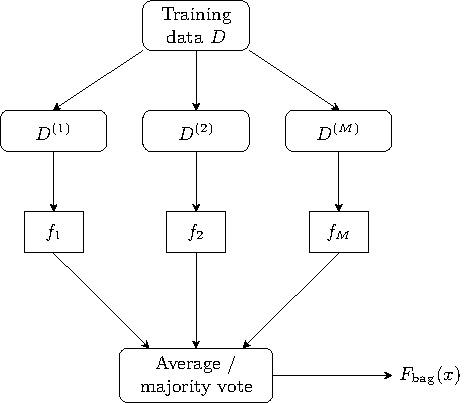
\includegraphics{../../tikz/8/6.pdf}
\end{figure}

\subsection{Random Forests}

Random Forests specialize bagging to decision trees, and further inject
randomness at the \emph{feature} level to decorrelate the trees.

\begin{definition}[Random Forest]
    A Random Forest is an ensemble of decision trees trained with two sources
    of randomness:
    \begin{enumerate}
        \item \textbf{Bootstrap sampling of data.}
        For each tree $m$, sample a bootstrap dataset $D^{(m)}$ from $D$.
        \item \textbf{Random feature selection at each split.}
        When splitting a node, instead of considering all features, randomly
        select a subset $\mathcal{F}$ of features (of size $d_{\mathrm{sub}}$),
        and choose the best split only among features in $\mathcal{F}$.
    \end{enumerate}
    The final prediction aggregates all trees by majority vote or averaging,
    as in bagging.
\end{definition}

The additional randomness in feature selection has two important effects:
\begin{itemize}
    \item It reduces the correlation between different trees, which
    strengthens the variance reduction effect of averaging.
    \item It forces each tree to explore different feature combinations,
    sometimes discovering useful patterns that a single greedy tree might miss.
\end{itemize}

In practice, Random Forests are strong general-purpose models with relatively
few hyperparameters.  Common choices include:
\begin{itemize}
    \item the number of trees $M$ (often in the hundreds),
    \item the maximum depth of each tree,
    \item the number of features $d_{\mathrm{sub}}$ considered at each split
    (e.g., $\sqrt{d}$ for classification, where $d$ is the total number of
    features).
\end{itemize}

\begin{remark}[Out-of-Bag Evaluation]
    In each bootstrap sample $D^{(m)}$, roughly a fraction $1-1/e\approx 0.63$
    of the original training points are included, and the remaining points are
    left out.  For any training example, we can average the predictions of all
    trees that did \emph{not} see this example during training; this is called
    the \emph{out-of-bag} prediction.  Aggregating these predictions over the
    training set provides an internal estimate of the generalization error,
    without using a separate validation set.
\end{remark}

\subsection{Boosting}

While bagging focuses on variance reduction by averaging many independent
learners, boosting builds an ensemble \emph{sequentially}.  Each new learner
tries to correct the mistakes of the current ensemble, effectively turning a
collection of weak learners into a strong one.

\begin{definition}[Boosting (High-Level View)]
    Given a training set $D = \{(x_i,y_i)\}_{i=1}^n$, boosting maintains an
    ensemble predictor
    \begin{equation}
        F_0(x) \equiv 0,\qquad
        F_M(x) = \sum_{m=1}^M \alpha_m f_m(x),
    \end{equation}
    where each $f_m$ is a base learner (often a shallow tree) and the weights
    $\alpha_m$ control their influence.
    
    At iteration $m$, boosting chooses $f_m$ to focus on the current residual
    errors or misclassified examples of $F_{m-1}$, and then updates the ensemble
    to $F_m$.
\end{definition}

One classical example is AdaBoost for binary classification.  It maintains a
distribution of weights over training samples, gives higher weights to
misclassified points, and fits a new weak learner to this reweighted dataset at
each iteration.

\begin{remark}[Boosting vs.\ Bagging]
    \begin{itemize}
        \item Bagging trains base learners \emph{in parallel} on resampled
        datasets and primarily reduces variance.
        \item Boosting trains base learners \emph{sequentially}, focusing on
        difficult samples, and can reduce both bias and variance, but is also
        more prone to overfitting if not regularized (e.g., via tree depth,
        learning rate, or early stopping).
    \end{itemize}
    Modern implementations such as Gradient Boosting Trees and XGBoost can be
    viewed as performing a form of functional gradient descent in function
    space, where each tree fits the negative gradient of the loss with respect
    to the current ensemble prediction.
\end{remark}

\begin{figure}[h]
    \centering
    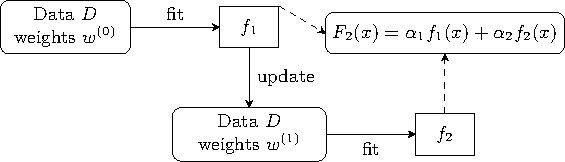
\includegraphics{../../tikz/8/7.pdf}
\end{figure}

\begin{note}
    From a geometric perspective, both Random Forests and boosting-based tree
    ensembles can be seen as constructing a complex, highly nonlinear decision
    boundary by patching together many simple, axis-aligned splits.  Whereas a
    single tree corresponds to a small set of such partitions, an ensemble can
    carve out increasingly intricate decision regions, often achieving
    state-of-the-art performance on tabular data.
\end{note}

\end{document}
